
\section*{Introduction}

In the present work, we replicate the results of Young et al. 2001 ``Reproductive pair correlations and the clustering of organisms'' \cite{young_reproductive_2001}, an analysis of the formation of aggregates in an otherwise homogeneous environment mimicking marine small-scale hydrodynamics. Using an individual-based model of independent, random-walking particles (also called ``Brownian bugs''), they show that reproduction by fission in a turbulent \cite{tennekes1972first} and viscous flow leads to the formation of elongated clusters. Spatial patterns therefore depart from the usual, homogeneous solution of the advection-diffusion-reaction equation for a large population. \\

Due to their size, phytoplankton organisms experience a mostly viscous environment in a laminar shear field, with random but homogeneous changes in directions due to turbulence  \citep{dusenbery2009living, peters_effects_2000}. Reproduction and limited movement of daughter cells, which occur at the phytoplankton scale, interact with these hydrodynamics processes and can lead to aggregates.  In this context, a better understanding of the interactions between demography and small-scale hydrodynamics could provide further explanation for observed spatial distribution of phytoplankton species, and perhaps even their coexistence. This motivated us to revisit Young et al. 2001 \cite{young_reproductive_2001}. \\

In addition to replicating the numerical and mathematical results of Young et al. 2001, we also wished to present the mathematical derivations that were missing from the original paper, which should make this replication article more accessible to most readers, especially those without a fluid mechanics background. 
%(see \cite{tennekes1972first} if further clarification on hydrodynamics phenomena is required).} 

\section*{Brownian bug model}
The Brownian bug model is defined as an individual-based model in continuous space and time, here presented in its 2D formulation. For efficient computer simulation, it is implemented in discrete time \cite{young_reproductive_2001}. Each particle is characterized by the vector of its Cartesian coordinates $\boldsymbol{x}=\begin{pmatrix} 
      x_1\\ 
      x_2 
\end{pmatrix}$ and its original position on the y-axis at $t=0$ (a child particle inherits this attribute), this last characteristic being used only for representation purposes. Space is a $L\times L$ square with periodic boundary conditions. Each timestep, of duration $\tau$, is divided into three substeps: (1) demographic processes, (2) diffusion, and (3) advection. \\

Demographic processes take place during the first substep (1). Each organism has a fixed probability ($p$) of reproducing, dying ($q$), or remaining unchanged ($1-p-q$). When an individual reproduces, a new organism appears on top of the parent. In the following, $p=q=0.5$. Diffusion is then modeled as a Brownian motion (2), i.e. $\boldsymbol{x'}(t)=\boldsymbol{x}(t)+\delta\boldsymbol{x}(t)$ where each component of $\delta\boldsymbol{x}(t)$ follows a Gaussian distribution $\mathcal{N}(0,\Delta)$ where $D~=~\frac{\Delta^2}{2\tau}$ is the diffusivity. The discrete-time Markov chain presented here approximates the continuous-time Brownian bug model, which can be thought of as a spatial birth-death or branching process (described in the Supplementary Material), step (1) being referred to in Young et al. \cite{young_reproductive_2001} as a Galton-Watson process. Finally, (3) the turbulent flow governing advective stirring follows the Pierrehumbert random map \citep{pierrehumbert_tracer_1994}.

\begin{eqnarray}
 x_1(t+\tau)&=&x'_1(t)+(U\tau/2)\cos[kx'_2(t)+\phi(t)] \label{eq:map1} \\
 x_2(t+\tau)&=&x'_2(t)+(U\tau/2)\cos[kx_1(t+\tau)+\theta(t)] \label{eq:map2}
 \label{eq:pierrehumbert}
 \end{eqnarray}

 where $\phi(t)$ and $\theta(t)$ are random phases uniformly distributed between 0 and $2\pi$, $k~=~2\pi/L$ and $U$ is the stretching parameter. \\
 
Unless otherwise specified, each simulation is initialized with $N_0=20,000$ particles uniformly distributed in a $1\times 1$ square and run for 1000 timesteps. 
 
% \subsection*{Relation with the advection-diffusion-reaction approximation} 
% In continuous time, the distribution of particles in conditions similar as those described in the Brownian bug model can be approximated by the advection-diffusion-reaction (ADR) equation. 
% 
% \begin{equation}
% \frac{dC}{dt}=D\nabla^2 C+(\lambda-\mu)C
% \label{eq:ADR}
% \end{equation}
% 
% where $C$ is the concentration of particles, $\lambda$ is the growth rate ($\lambda=p/\tau$)  and $\mu$ is the death rate ($\mu=q/\tau$). When $\lambda=\mu$, the solution of eq. \ref{eq:ADR} is $C(\boldsymbol{x},t)=C_0$ where $C_0$ is the initial uniform concentration. To compare this theoretical distribution to the actual distribution, the Brownian bug model is run without the advection component ($U=0$). While the Brownian bug model is a discrete-time model, we consider $\tau \leftarrow 0.1$. \\
% 
% To assess the effect of the turbulent motion, the model is also run without its demographic component, but with advection and diffusion.
\subsection*{Pair density function $G(r,t)$}

The pair density function $G(\boldsymbol{x}_i,\boldsymbol{x}_j,t)$ is defined so that $G(\boldsymbol{x}_i,\boldsymbol{x}_j,t)dA_1dA_2$ is the probability of finding a pair of Brownian bugs with one member in the area $dA_1$ around $\boldsymbol{x}_i$ and the other in the area $dA_2$ around $\boldsymbol{x}_j$. Defining $\boldsymbol{\xi}=\boldsymbol{x}_i-\boldsymbol{x}_j$,  $G(\boldsymbol{\xi},t)$ is actually called the pair correlation function in \cite{young_reproductive_2001}. The radial density function $g(r,t)$ is defined as $G(\boldsymbol{\xi},t)=C^2g(r,t)$ where $C$ is the concentration of bugs and $r=|\boldsymbol{\xi}|$. As the pair correlation disappears when $r\rightarrow\infty$, $g\rightarrow 1$. \\

\subsubsection*{Derivation of $G(r,t)$}

All details of the derivation of $G(r,t)$ are to be found in the Supplementary Material. We finally obtain:

\begin{equation}
\frac{\partial G}{\partial t}=2Dr^{1-d}\frac{\partial}{\partial r}\left(r^{d-1}\frac{\partial G}{\partial r}\right)+2(\lambda-\mu)G+\gamma r^{1-d}\frac{\partial}{\partial r}\left(r^{d+1}\frac{\partial G}{\partial r}\right)+2\lambda C\delta(\boldsymbol{\xi})\label{eq:eq_2_Young_total}
\end{equation}
where $\lambda$ is the birth rate ($p=\lambda\tau$) and $\mu$ is the death rate ($q=\mu\tau$). \\

We focus on the case $d=2$ and $\lambda=\mu$, which means Eq.~\ref{eq:eq_2_Young_total} can be reduced to

\begin{equation}
\frac{\partial G}{\partial t}=\frac{2D}{r}\frac{\partial}{\partial r}\left(r\frac{\partial G}{\partial r}\right)+\frac{\gamma}{r}\frac{\partial}{\partial r}\left(r^{3}\frac{\partial G}{\partial r}\right)+2\lambda C\delta(\boldsymbol{\xi}).\label{eq:eq_2_Young_reduced}
\end{equation}

The value of $\gamma$ is computed from simulations (see Supplementary Material).

\subsubsection*{Analytical solution with advection}

CP and FB could only find the analytical solutions of $G(r,t)$ with and without advection with the indications of WY. In the presence of advection ($\gamma\neq0$), a steady-state solution
can be found; without advection, there is no steady-state and the solution changes through time. Let us first examine the steady-state solution, given by:

\begin{align}
  &  \frac{2D}{r}\frac{\partial}{\partial r}\left(r\frac{\partial G}{\partial r}\right)+\frac{\gamma}{r}\frac{\partial}{\partial r}\left(r^{3}\frac{\partial G}{\partial r}\right)+2\lambda C\delta(\boldsymbol{\xi})\nonumber & = & & 0 \\
\Leftrightarrow & 2\pi r\left(\frac{2D}{r}\frac{\partial}{\partial r}\left(r\frac{\partial G}{\partial r}\right)+\frac{\gamma}{r}\frac{\partial}{\partial r}\left(r^{3}\frac{\partial G}{\partial r}\right)+2\lambda C\delta(\boldsymbol{\xi})\right)\nonumber & = & & 0 \\
 \Leftrightarrow  & 2\pi\left(2D\frac{\partial}{\partial r}\left(r\frac{\partial G}{\partial r}\right)+\gamma\frac{\partial}{\partial r}\left(r^{3}\frac{\partial G}{\partial r}\right)\right)+2\pi r2\lambda C\delta(\boldsymbol{\xi}) & = & & 0.\label{eq:steady_state}
\end{align}

We can then integrate Eq.~\ref{eq:steady_state} over a small area centered on a particle, with radius $\rho$. Let us first note that

\begin{align}
& \int_{\mathbb{R}^{2}}\delta(\boldsymbol{x})d\boldsymbol{x} & & = & & 1\nonumber \\
\Leftrightarrow & \int_{0}^{2\pi}\int_{0}^{\rho}\delta(r)\delta(\theta)rdrd\theta & & = & & 1\nonumber \\
\Leftrightarrow & 2\pi\int_{0}^{\rho}\delta(r)rdr & & = & & 1.\label{eq:delta_integration}
\end{align}

Using Eq.~\ref{eq:steady_state} and \ref{eq:delta_integration}, we can integrate between 0 and $\rho$, 

\begin{align}
 & & 0 & & = & & 2\pi\left(2D\rho\frac{\partial G}{\partial \rho}+\gamma\rho^{3}\frac{\partial G}{\partial \rho}\right)+2\lambda C\nonumber \\
\Leftrightarrow & & \frac{\partial G}{\partial \rho} & & = & & -\frac{1}{2\pi}\frac{2\lambda C}{2D\rho+\gamma\rho^{3}}.\label{eq:deriv_G_r}
\end{align}

Eq.~\ref{eq:deriv_G_r} can now be integrated between $\rho$ and $\infty$, knowing that $G(\infty)=C^{2}$:

\begin{equation}
 C^{2}-G(\rho) = -\frac{1}{2\pi}{\displaystyle \int_{\rho}^{\infty}}\frac{2\lambda C}{2Dr+\gamma r^{3}}dr.\label{eq:deriv_G_r_int1}
\end{equation}

Using the variable change $u=\frac{2D}{r^{2}}+\gamma$, with $du=\frac{-4D}{r^{3}}dr$,
the integral writes
\begin{equation}
\begin{array}{ccc}
G(\rho) & = & C^{2}+\frac{\lambda C}{\pi}{\displaystyle \int_{\frac{2D}{\rho^{2}}+\gamma}^{\gamma}}\frac{1}{r^{3}u}\frac{r^{3}}{-4D}du\\
 & = & C^{2}-\frac{\lambda C}{4\pi D}\left[\ln u\right]_{\frac{2D}{\rho^{2}}+\gamma}^{\gamma}\\
 & = & C^{2}-\frac{\lambda C}{4\pi D}\left(\ln(\gamma)-\ln\left(\frac{2D}{\rho^{2}}+\gamma\right)\right)\\
 & = & C^{2}+\frac{\lambda C}{4\pi D}\ln\left(\frac{2D+\gamma \rho^{2}}{\gamma \rho^{2}}\right).
\end{array}
\end{equation}
Finally, the pair correlation function $g=G/C^{2}$ is defined as
\begin{equation}
g(r)=\frac{\lambda}{4\pi DC}\ln\left(\frac{2D+\gamma r^{2}}{\gamma r^{2}}\right)+1.
\end{equation}

\subsubsection*{Analytical solution without advection}

When $U=0$, $\gamma=0$ and there is no steady solution in 2D. We can get back to Eq.~\ref{eq:eq_2_Young_reduced}:

\begin{equation}
\frac{\partial G}{\partial t}=\frac{2D}{r}\frac{\partial}{\partial r}\left(r\frac{\partial G}{\partial r}\right)+2\lambda C\delta(\boldsymbol{\xi}).\label{eq:g_without_advection}
\end{equation}

Assuming an isotropic environment (and switching to the Cartesian coordinate system), this means

\begin{equation}
\frac{\partial G}{\partial t}-2D\Delta G=2\lambda C\delta(\boldsymbol{\xi})
\end{equation}

where $\Delta=\nabla^{2}$ is the Laplacian operator. \\

We therefore have 

\begin{equation}
\mathcal{L}G(\boldsymbol{\xi},t)=2\lambda C\delta(\boldsymbol{\xi})\label{eq:LG_lambda}
\end{equation}

where $\mathcal{L}$ is the linear differential operator $\partial_{t}-2D\Delta$. \\

We can use a Green's function $H$, defined with $\mathcal{L}H=\delta(\boldsymbol{\xi},t)=\delta(\boldsymbol{\xi})\delta(t)$. \\

By definition, we know that $G(y)=\int H(y,s)2\lambda C\delta(s)ds$
(where $y=(\boldsymbol{\xi},t)$) is a solution to Eq.~\ref{eq:LG_lambda}.

\begin{align}
 G(\boldsymbol{\xi},t)  =  & 2\lambda C\int_{\mathbb{R}^{2}}\int_{0}^{t}H(\boldsymbol{\xi}-\boldsymbol{\xi}',t')\delta(\boldsymbol{\xi}')d\boldsymbol{\xi}'dt'\nonumber \\
 = &  2\lambda C\int_{0}^{t}H(\boldsymbol{\xi},t')dt'.\label{eq:g_int_H}
\end{align}

Eq.~\ref{eq:g_int_H} can be used in Eq.~\ref{eq:g_without_advection}:

\begin{align}
 & \frac{\partial}{\partial t}\left(2\lambda C\int_{0}^{t}H(\boldsymbol{\xi},t')dt'\right) & & = & & 2D2\lambda C\Delta\int_{0}^{t}H(\boldsymbol{\xi},t')dt'+2\lambda C\delta(\boldsymbol{\xi})\\
\Leftrightarrow & \int_{0}^{t}\left(\frac{\partial H(\boldsymbol{\xi},t')}{\partial t'}-2D\Delta H(\boldsymbol{\xi},t')\right)dt' & & = & & \delta(\boldsymbol{\xi})\\
\Leftrightarrow & \int_{0}^{t}\delta(\boldsymbol{\xi})\delta(t')dt' & & = & & \delta(\boldsymbol{\xi})
\end{align}

which is true. \\

A solution for the Green's function using $\mathcal{L}=\partial_{t}-2D\Delta$
in 2 dimensions is 

\begin{equation}
H(r,t)=\frac{1}{4\pi2Dt}\exp\left(\frac{-r^{2}}{4\times2Dt}\right). 
\end{equation}

$G(r,t)$ can then be computed:

\begin{equation}
G(r,t)=2\lambda C\left[\frac{E_1 \left(\frac{r^{2}}{8Dt'}\right)}{8D\pi}\right]_{0}^{t}\label{eq:G_r_t}
\end{equation}

where $E_1(x)=\int_x^\infty \frac{e^{-t}}{t}dt$ is the exponential integral. Using $G(r,0)=C^{2}$ and
$\lim_{x\rightarrow+\infty}E_1~=~0$ in Eq.~\ref{eq:G_r_t}, we finally obtain

\begin{equation}
G(r,t)=\lambda C\frac{E_1\left(\frac{r^{2}}{8Dt}\right)}{4D\pi}+C^{2}
\end{equation}

\begin{equation}
\Leftrightarrow g(r,t)=\frac{\lambda}{C}\frac{E_1\left(\frac{r^{2}}{8Dt}\right)}{4D\pi}+1.
\end{equation}

\section*{Results}

We were able to reproduce the three figures of Young et al. \cite{young_reproductive_2001} highlighting the spatial distributions of Brownian bugs.\\

In Fig. \ref{fig:spatial_fig1}, the model has been run without the advection component and we can see the clumping of organisms due to reproduction. In Fig. \ref{fig:spatial_fig2} a), the model has been run without its demographic component, but with advection and diffusion, confirming that hydrodynamics alone cannot ensure cluster formation, while in Fig.  \ref{fig:spatial_fig2} b), advection, diffusion and demography are present, in which case organisms form elongated aggregates.\\
  
Fig. \ref{fig:pcf_Fig3} proved much more challenging. Retrieving the analytical solutions of Eq.~\ref{eq:eq_2_Young_reduced} was difficult as there was no other equation than Eq. \ref{eq:eq_2_Young_total} in the original paper. We also encountered issues when computing the pair correlation functions on simulations: for large values of $r/\Delta$, we observed zero values (absent pairs) of the pcf when $U=0$. This is a sampling effect as pcf values get very low for large distances without advection, even though we multiplied the study area by 10 to produce Fig.  \ref{fig:pcf_Fig3} and counter such effects. Despite the missing values, we can confirm that simulated and analytical pcf match (Fig. \ref{fig:pcf_Fig3}), with a slight underestimation by the simulations. The numerical pcf also got closer to 1 than the analytical predictions for large values of $r$.

\begin{figure}[H]
\begin{center} 
 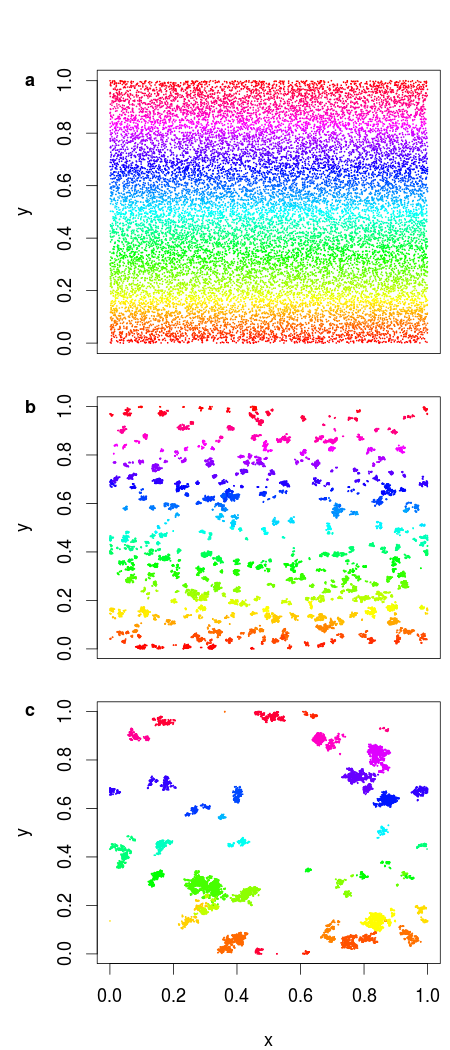
\includegraphics[width=0.86\textwidth]{../code/figure/spatial_distribution_Fig1.png}
  \caption{Distribution of Brownian bugs at different times in a simulation with $\Delta=10^{-3}$ and $U=0$: initial conditions with a Poisson spatial distribution (a), $t=100\tau$ (b) and $t=1000\tau$ (c). Each particle is identified by a color which corresponds to the initial position on the y-axis of its ancestor at $t=0$.}
  \label{fig:spatial_fig1}
\end{center}
  \end{figure}

\begin{figure}[H]
\begin{center}
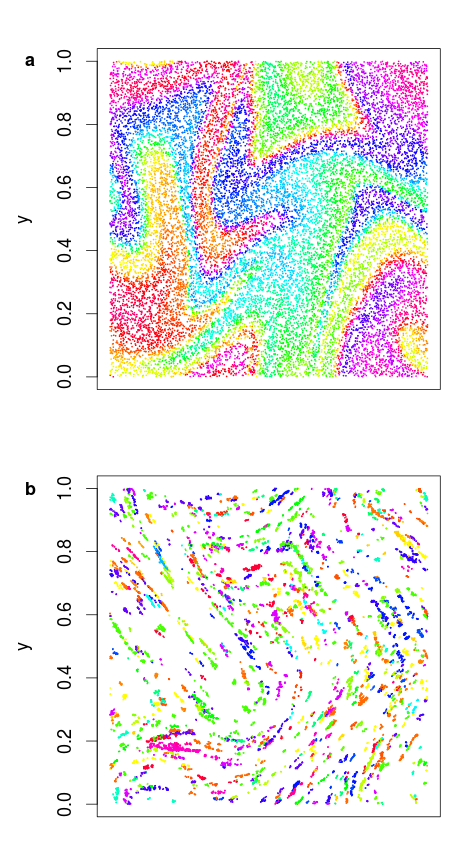
\includegraphics[width=0.99\textwidth]{../code/figure/spatial_distribution_Fig2.png}
  \caption{Distribution of Brownian bugs in a simulation with advection and $\Delta=10^{-3}$, $U\tau/2=0.1$: without demographic processes at $t=30\tau$ (a), and with demographic processes at $t=1000\tau$ (b). Each particle is identified by a color which corresponds to the initial position on the y-axis of its ancestor at $t=0$.}
  \label{fig:spatial_fig2}
\end{center}
  \end{figure}


\begin{figure}[H]
\begin{center}
 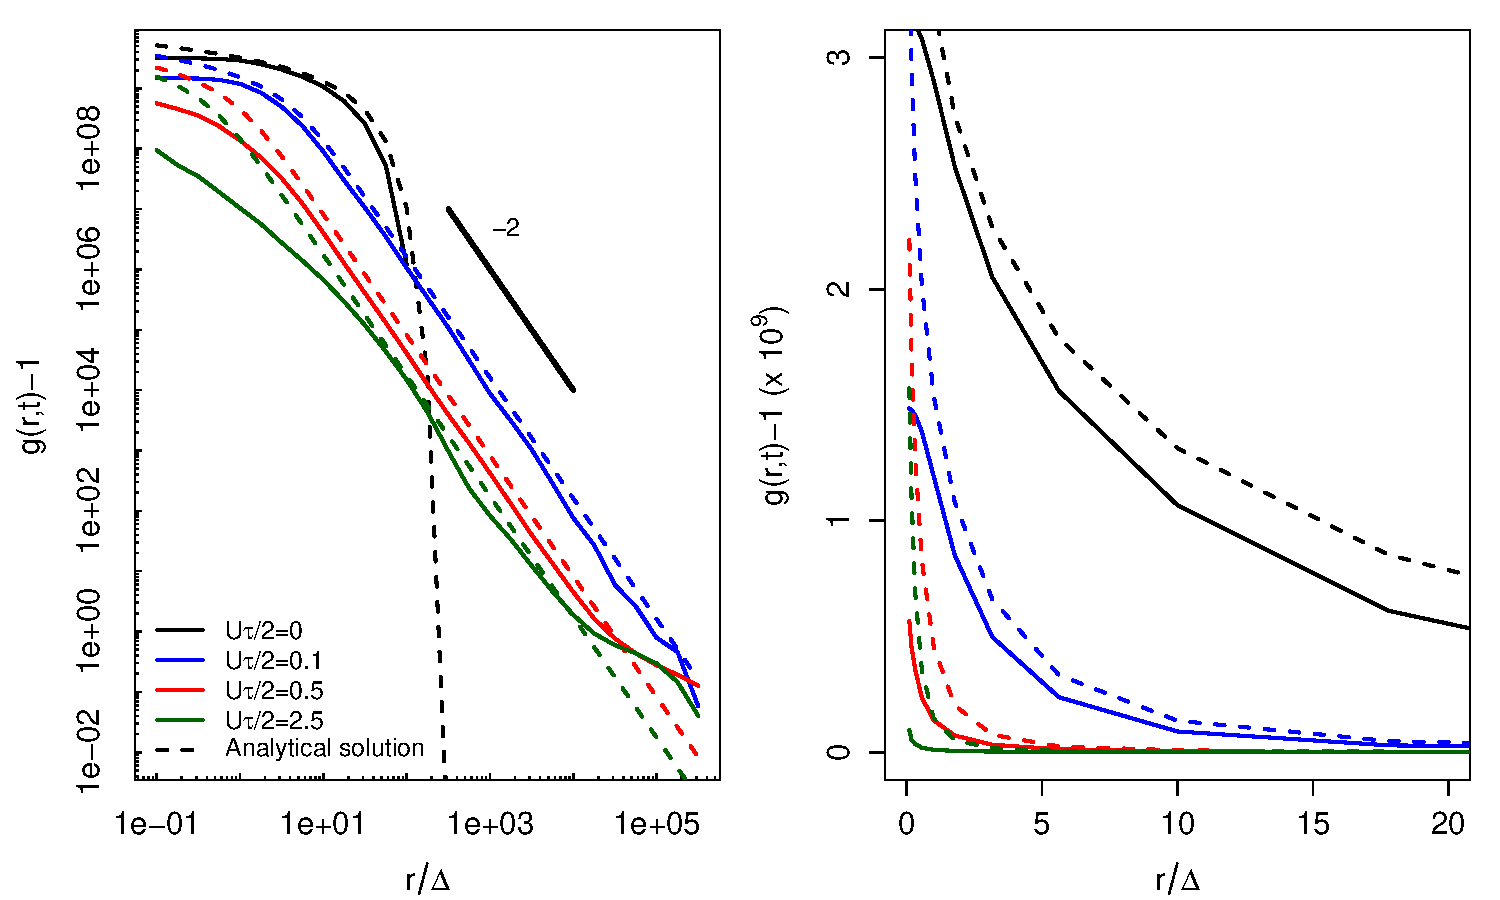
\includegraphics[width=0.99\textwidth]{../code/figure/pcf_test_Utot_modif_dx_dp.pdf}
 \caption{Logarithmic (a) and linear (b) plots of $g(r,t)$ versus $r/\Delta$, with $\Delta=10^{-7}$ and $U\tau/2=0,0.1,0.5,2.5$ at $t=1000\tau$. To compute simulation-based values of $g(r)$ with a large number of points ($N_0=200,000$) and avoid sampling issues, we replicated the $1\times 1$ square $10$ times, so that its length is $\sqrt{10}$ while keeping $L=1$ and $k=2\pi/L$ in eq. \ref{eq:map1} and \ref{eq:map2}. Solid lines result from simulations, dotted lines correspond to analytical solutions and the solid grey line indicates the $r^{-2}$ scaling predicted by Eq.~\ref{eq:eq_2_Young_total}.}
  \label{fig:pcf_Fig3}
\end{center}
  \end{figure} 
 
\section*{Discussion}

We successfully replicated both the numerical results and analytical solutions of Young et al. \citep{young_reproductive_2001}. Even though stochasticity prevents us from replicating exactly the same spatial point patterns as those seen in the original Fig. \ref{fig:spatial_fig1} and Fig. \ref{fig:spatial_fig2}, we considered the patterns to be close enough to validate the replication. Fig. \ref{fig:pcf_Fig3} was also very close to the one shown in the original article, despite a slight underestimation of the pcf in simulated data.\\

The most challenging part of the replication was actually not to replicate the numerical results, but to find back the analytical expression of the pair density function $G(r,t)$ dynamics from first principles. How to derive such dynamics was indeed briefly explained in words in the original article, but the many intermediate steps involved (see Supplementary Material) make the additional mathematical derivations presented here worthwhile in our opinion. In addition to providing critical information to CP and FB regarding how to obtain the pair correlation dynamics, WY also communicated the required mathematical steps to find back the analytical solutions for $G(r,t)$ plotted in Fig. \ref{fig:pcf_Fig3}. We hope that the additional material on the derivation of $G(r,t)$ dynamics (as Supplementary Material) as well as the provided analytical solutions of such dynamics (now presented in the main text) will help readers through both the original and replication articles. \\

The original article did not provide quantitative values exactly matching marine microbes ecology; we thus wondered about the time and spatial scales that could be used for a realistic phytoplankton model. The length of the square side, $L$, is defined roughly as the Kolmogorov scale \citep{tennekes1972first}, the scale at which viscosity starts dominating turbulence  (we use $L= 1$ cm as an upper bound). Here, we consider $k$ the smallest wavenumber corresponding to the largest length scale $L$, i.e. $k=2\pi/L$. The chosen length scale defines the Reynolds number which then allows to obtain $U$, the velocity difference between two points separated by a distance $L$.  
 
\begin{eqnarray}
 \text{Re} & = &\frac{U}{k\nu}\\
\Rightarrow 1 & = & \frac{UL}{2\pi\nu}\\
\Leftrightarrow U & = &\frac{2\pi\nu}{L}
\end{eqnarray}
% 
where $\nu=10^{-6} \text{ m}^{2}~\text{s}^{-1}$ is the kinematic viscosity for water. These numerical values lead to $U=6.3\times10^{-4} \text{ m~s}^{-1}$. Note that $U$ is the speed in the frame of reference of the small square area considered here, which might itself be embedded within larger spatial structures (e.g., large eddies) moving at higher speeds in the ocean or any large waterbody.\\

To determine the diffusivity of small organisms, we use the Stokes-Einstein equation \citep{einstein1905molekularkinetischen}:

\begin{equation}
 D=\frac{RT}{N_{A}}\frac{1}{6\pi\eta a}
\end{equation}

where $R=8.314$ J~K$^{-1}$~mol$^{-1}$ is the molar gas constant, $T=293$ K is the temperature of the environment, $N_{A}=6.0225\times10^{23}$ is Avogadro's number, $\eta=10^{-3}\text{ m}^{-1}~\text{kg~s}^{-1}$ is the viscosity of water and $a$ is the radius of the organism considered. We apply this formula to microphytoplankton organisms of diameter 50 \textmu m, keeping $\tau$ outside of the equation for now:

\begin{eqnarray}
\Delta & = & \sqrt{2D\tau}\\
  &= & \sqrt{\frac{RT}{N_{A}}\frac{\tau}{3\pi\eta a}}\\
&=& \sqrt{\frac{8.314\times293}{6.0225\times10^{23}}\frac{1}{3\pi\times10^{-3}\times25\times10^{-6}}}\sqrt{\tau}\\
 & = & 1.3 \times 10^{-7} \sqrt{\tau} \text{ m.}
\end{eqnarray}

To compute $\tau$, we can consider a phytoplankton doubling rate of $1$ d$^{-1}$ \citep{bissinger_predicting_2008}, which means, with $p=0.5$, that $\tau=0.5$ d.\\

This leads to $U\tau/2\approx 5.4\times10^{3} \text{ cm~d}^{-1}$ and $\Delta \approx 5\times10^{-5}$ cm. These two values are much higher than those used in Fig. \ref{fig:pcf_Fig3} ($0.1<U\tau/2<2.5$ and $\Delta=10^{-7}$). A thorough discussion of the parameters is therefore necessary before extrapolating these results to real phytoplanktonic systems. \\

As the Brownian bug model is currently fairly theoretical in its 2D formulation, a logical next step would be to consider similar dynamics in a 3D-model, which would render the comparison to real data easier. Using actual concentrations of phytoplanktonic organisms (e.g., diatoms), between 10$^3$ and 10$^6$ C/L, this would lead to 1 to 10$^3$ organisms if we kept $L$ = 1 cm. We might therefore need to increase the size of the considered square, or apply the model to small bacteria only. With a closer match between field and simulated concentrations, the model could provide us with a better picture of the likely fine-scale spatial structure of phytoplanktonic populations. 

\section*{Acknowledgements}
We are grateful to Francesco Turci for comments and to Rajesh Singh for detailed feedback and code suggestions. 

%Another to look at this velocity is to consider the Reynolds number ($Re \approx 1$ in this case); we have $Re  = V L_c / \nu$ where $V$ is the fluid characteristic speed, $L_c$ the spatial scale, and $\nu = 10^{-6} m^2/s$ for water. If $L_c = L = 1$ cm, we have $V = 10^{-4} m/s = 0.1 mm/s$. 

%Stuff that we could discuss: scales? Pierrehumber formulation for turbulence?

